\section{Einleitung}

Im Rahmen der vorliegenden Arbeit wurde ein Modell in den Raytracer pbrt integriert, welches die Verzerrungen durch reale Objektive simuliert. Liegen gemessene Verzerrungsparameter einer Optik vor, können diese vor dem Rendervorgang übergeben werden und es wird eine physikalisch korrekte Berechnung dieser Verzerrung durchgeführt.
Alle Ergebnisse und die genutzten Test-Szenen finden sich im folgendem Git-Repository: \url{https://github.com/Phenylalaninquelle/distortionCamera}. Die Implementierung der Klasse kann unter \url{https://github.com/Phenylalaninquelle/pbrt-v3} über den Tag \texttt{submissionCommit} abgerufen werden.

\section{Theorie}

\subsection{Was ist ein Raytracer?}\label{sec:Raytracer}

Dazu muss zuerst der Begriff \textit{Rendering} erklärt werden. Dieser beschreibt ganz allgemein den Prozess, der aus der Beschreibung einer dreidimensionalen Szene ein zweidimensionales Bild erzeugt. Dazu sind zahlreiche Algorithmen notwendig, welche beispielsweise Geometrien modellieren, Objekte animieren oder Texturen erzeugen und die Ergebnisse hiervon an den Render-Prozess weitergeben, um diese sichtbar zu machen. 

Um eine dreidimensionale Szene in ein Bild abzubilden, kann sich des Raytracing-Algorithmus bedient werden. Wie sich bereits aus dem Begriff ableiten lässt, werden dabei die Pfade einzelner \glqq Lichtstrahlen\grqq{ }verfolgt, bis diese auf eine Oberflächen treffen und es beispielsweise zu einer Reflexion kommt. In diesem Fall würden nun die Richtungen und Intensitäten der reflektierten Strahlen bestimmt und diese weiter verfolgt.
Da dabei nur diejenigen Strahlen von Interesse sind, welche auch tatsächlich auf den virtuellen Bildsensor treffen und für den Helligkeits- und Farbwert eines Pixels im Bild einen Beitrag leisten, verfolgen Raytracer die Strahlen in umgekehrter Richtung. Es werden also Strahlen am Bildsensor erzeugt und in die Szene geschickt, bis sie mit einer Oberfläche interagieren. Auf diese Weise werden alle Lichtquellen identifiziert, die für die Berechnung des Helligkeits- und Farbwertes des gerade betrachteten Pixels relevant sind \cite{pbrt_book}. 

Der in dieser Arbeit genutzte Raytracer ist \textit{pbrt}\cite{pbrt}. Dieser hat den Anspruch, das Rendering \textit{physically based}, also möglichst physikalisch korrekt, durchzuführen. Aus diesem Grund sind hier viele fundamentale Gleichungen der Optik implementiert und Phänomene werden somit korrekt berechnet. Im Gegensatz dazu stehen Raytracer, welche für Animationsfilme oder Computerspiele genutzt werden. Hier soll das Endergebnis möglichst \textit{gut} aussehen, ohne unbedingt physikalisch korrekt zu sein. 

Trotz des Anspruchs von pbrt, möglichst physikalisch korrekte Resultate zu erzeugen, sind manche optische Phänomene noch nicht implementiert. So besteht im Moment noch keine Möglichkeit, die optischen Verzerrungen nachzubilden, welche von allen realen Optiken verursacht werden.
In der vorliegenden Arbeit wird ein neues Kameramodell in den frei verfügbaren Quellcode von pbrt eingefügt, welches gemessene Verzerrungen von Optiken berechnet.

\subsection{Verzerrung}

Die Verzerrungen, welche von realen Optiken verursacht werden, führen dazu, dass in der Realität ungekrümmte Linien in der zweidimensionalen Abbildung gekrümmt erscheinen. Dies geschieht dadurch, dass Punkte im aufgenommenen Bild verschoben abgebildet werden und zwar umso stärker, je weiter sie von der optischen Achse entfernt sind. Besonders gut lässt sich dieser Effekt mit Weitwinkelobjektiven an Hausfassaden beobachten. 
Genauer wird dabei zwischen Kissen- und Tonnenverzeichnung unterschieden. In Abbildung \ref{fig:distortionBarrel} und \ref{fig:distortionPinc} wird deutlich, dass bei der Kissenverzeichnung (auch positive Verzeichnung) die Bildpunkte von der optischen Achse weg verschoben werden, während der Abstand der Bildpunkte zur optischen Achse bei der Tonnenverzeichnung (auch negative Verzeichnung) kleiner wird. Durch die bereits erwähnte Zunahme dieses Effekts mit steigendem Radius zur optischen Achse, erfahren in der Realität gerade Linien eine Krümmung \cite{smith2000modern}.

\begin{figure}[h]
	\begin{minipage}{.5\textwidth}
		\centering
		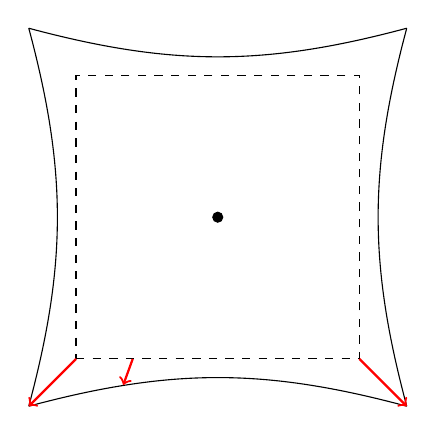
\begin{tikzpicture}[scale=0.6]
		% undistorted:
		\draw[black, dashed] (-3, -3) -- (3, -3) -- (3, 3) -- (-3, 3) -- (-3, -3);
		
		% distorted pincushion
		\draw (-4 ,-4) to[out=15,in=165] (4 , -4);
		\draw (4 ,-4) to[out=105,in=255] (4 , 4);
		\draw (4 ,4) to[out=195,in=-15] (-4 , 4);
		\draw (-4 ,4) to[out=285,in=75] (-4 , -4);
		
		% optical centre
		\filldraw 
		(0,0) circle (3pt);
		
		%distortion arrows
		\draw [red, ->, thick] (-3, -3) -- (-4, -4);
		\draw [red, ->, thick] (3, -3) -- (4, -4);
		\draw [red, ->, thick] (-1.8, -3) -- (-2., -3.55);
		
		\end{tikzpicture}
		\caption{Kissenverzeichnung}
		\label{fig:distortionBarrel}
	\end{minipage}
	\begin{minipage}{.5\textwidth}
		\centering
		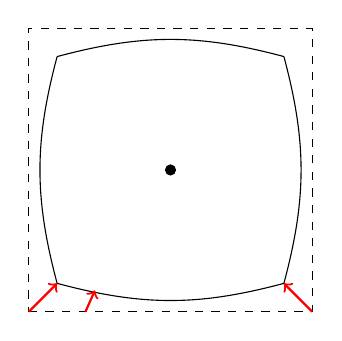
\begin{tikzpicture}[scale=0.6]
		% undistorted
		\draw[black, dashed] (-3, -3) -- (3, -3) -- (3, 3) -- (-3, 3) -- (-3, -3);
		
		%distorted barrel
		
		\draw (-2.4 ,-2.4) to[out=-15,in=-165] (2.4 , -2.4);
		\draw (2.4 ,-2.4) to[out=75,in=285] (2.4 , 2.4);
		\draw (2.4 ,2.4) to[out=165,in=15] (-2.4 , 2.4);
		\draw (-2.4 ,2.4) to[out=255,in=105] (-2.4, -2.4);
		
		% optical centre
		\filldraw 
		(0,0) circle (3pt);
		
		%distortion arrows
		\draw [red, ->, thick] (-3, -3) -- (-2.4, -2.4);
		\draw [red, ->, thick] (3, -3) -- (2.4, -2.4);
		\draw [red, ->, thick] (-1.8, -3) -- (-1.6, -2.55);
 	     
	    		
		\end{tikzpicture}
		\caption{Tonnenverzeichnung}
		\label{fig:distortionPinc}
	\end{minipage}
\end{figure}

\subsection{Lochkameramodell}\label{sec:pinhole}

Das einfachste Kameramodell, welches beim Rendern von Bildern genutzt werden kann, ist das Lochkameramodell, welches in Abbildung \ref{fig:pinholeCam} dargestellt ist. 
\begin{figure}[h]
	\centering
	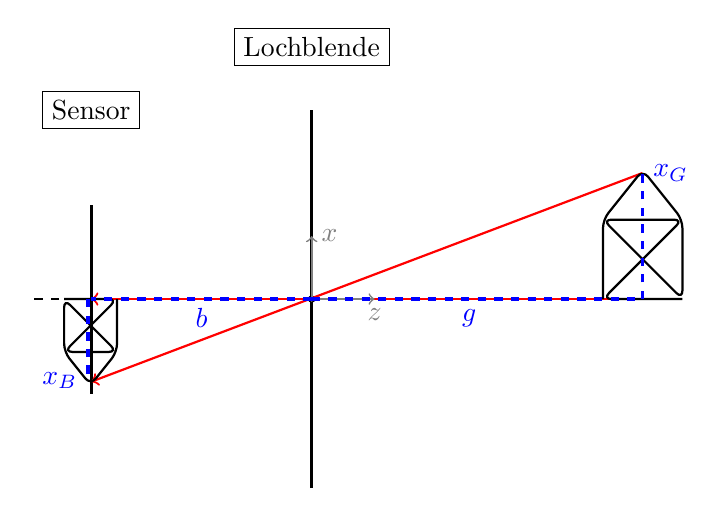
\begin{tikzpicture}[scale=0.4]
	
	% sensor
	\draw[very thick] (-7,-3) -- (-7, 3);
	% lochblende
	\draw (0,0) circle [radius=0.1];
	\draw[very thick] (0, -6) -- (0, -0.1);
	\draw[very thick] (0, 6) -- (0, 0.1);
	%optische Achse
	\draw[thin, dashed] (2, 0) -- (-9, 0);
	%Lichtstrahl Dach
	\draw[thick, red, ->] (10.5, 4) -- (-7, -21/8);
	%Lichtstrahl Boden
	\draw[thick, red, ->] (10.5, 0) -- (-7, 0);
	%Koordinatensystem
	\draw[semithick, gray, ->] (0,0) -- (0,2) node[right] {$x$};
	\draw[semithick, gray, ->] (0,0) -- (2,0) node[below] {$z$};
	%Beschriftung
	\node[draw] at (-7, 6) {Sensor};
	\node[draw] at (0, 8) {Lochblende};
	
	% Nikolaus echt
	\begin{scope}[shift={(9.25,0)}, scale=1.26]
	\draw[thick,rounded corners=3pt] (0,0) -- (0,2) -- (1,3.25) 
	-- (2,2) -- (2,0) -- (0,2) -- (2,2) -- (0,0) -- (2,0);
	\end{scope}
	
	% Nikolaus Abbildung
	\begin{scope}[shift={(-6.18,0)}, scale=0.84, rotate=180]
	\draw[thick,rounded corners=3pt] (0,0) -- (0,2) -- (1,3.25) 
	-- (2,2) -- (2,0) -- (0,2) -- (2,2) -- (0,0) -- (2,0);
	\end{scope}
	
	% ähnliche Dreiecke
	\draw [very thick, blue, dashed](-7.1, 0 )-- (-7.1, -2.6) node [left] {$x_B$};
	\draw [very thick, blue, dashed](10.5, 0 )-- (10.5, 4) node [right] {$x_G$};
	
	\draw [very thick, blue, dashed](0, 0 )-- (10.5, 0);
	\draw [blue] (5, -0.6 ) node {$g$};
	\draw [very thick, blue, dashed](0, 0 )-- (-7, 0);
	\draw [blue] (-3.5, -0.6 ) node {$b$};
	
	\end{tikzpicture}
	\caption{Lochkamera-Modell im zweidimensionalen Fall}
	\label{fig:pinholeCam}
\end{figure}
Alle Lichtstrahlen, welche auf den Sensor treffen, müssen die Blende durch das infinitesimal kleine Loch passieren. Durch Größe des Sensors und dessen Abstand zur Blende wird das Sichtfeld (auch FOV, Field of view) festgelegt.
Durch die Anwendung der Ähnlichkeitssätze für Dreiecke, kann aus den Koordinaten des Gegenstands (rechts der Lochblende) auf die Bildkoordinaten auf dem Sensor (links der Lochblende) geschlossen werden, wie in Abbildung \ref{fig:pinholeCam} für die x-Koordinate dargestellt ist \cite{pbrt_book}:

\begin{equation}
x_B = \frac{x_G \cdot b}{g}
\end{equation}

Wie bereits im Kapitel \ref{sec:Raytracer} erwähnt, treffen bei der Anwendung des Kameramodells im Raytracer jedoch keine Lichtstrahlen von außen in die Kamera. Vielmehr werden Lichtstrahlen am Sensor erzeugt und nach außen in die Szene geschickt, um nur diejenigen Strahlen zu berechnen, welche tatsächlich einen Beitrag für das zu rendernde Bild leisten.

\subsection{Integration der Verzerrung in den Raytracer}\label{sec:DistortionRaytracer}

%\subsubsection{Konzept ( Warum muss man invertieren? )}

%Das Lochkamera-Modell geht von einer infinitesimal kleinen Blendenöffnung aus. Einfallende Lichtstrahlen, die auf die Öffnung treffen, bewegen sich ungehindert in ihre Ausbreitungsrichtung weiter und treffen an einem Punkt $p_1$ auf den Kamerasensor (siehe blauer Strahl in Abbildung \ref{fig:model}).
Die Auswirkungen einer Linsenverzerrung sind in Abbildung \ref{fig:model} dargestellt. Der Lichtstrahl bewegt sich nicht mehr ungehindert in seiner Ausbreitungsrichtung weiter und trifft an einem Punkt $p_1$ auf den Kamerasensor (siehe blauer Strahl), sondern
wird an der Öffnung der Lochblende in einem bestimmten Maße abgeknickt und erreicht den Sensor am Punkt $p_2$ (roter Strahl). Die Funktion, die die normalisierten Pixelkoordinaten des unverzerrten Punktes $p_1$ auf die des verzerrten Punktes $p_2$ abbildet, bezeichnen wir mit $f$.
\begin{figure}[h]
	\centering
	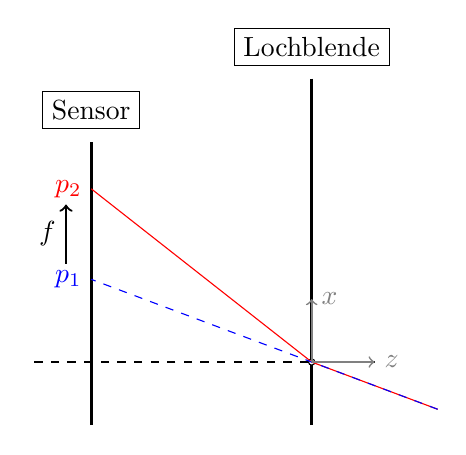
\begin{tikzpicture}[scale=0.4]

	% sensor
	\draw[very thick] (-7,-2) -- (-7, 7);
	% lochblende
	\draw (0,0) circle [radius=0.1];
	\draw[very thick] (0, -2) -- (0, -0.1);
	\draw[very thick] (0, 9) -- (0, 0.1);
	%optische Achse
	\draw[thin, dashed] (2, 0) -- (-9, 0);
	%abgelenkter Lichtstrahl
	\draw[red] (4, -1.5) -- (0, 0) -- (-7, 5.5) node[left] {$p_2$};
	%durchgehender Lichtstrahl
	\draw[blue, dashed] (4, -1.5) -- (-7, 21/8) node[left] {$p_1$};
	%Verzeichnungspfeil
	\draw[->, thick] (-7.8, 21/8 + 0.5) -- (-7.8, 65/16) node[left] {$f$} -- (-7.8, 5) ;
	%Koordinatensystem
	\draw[semithick, gray, ->] (0,0) -- (0,2) node[right] {$x$};
	\draw[semithick, gray, ->] (0,0) -- (2,0) node[right] {$z$};
	%Beschriftung
	\node[draw] at (-7, 8) {Sensor};
	\node[draw] at (0, 10) {Lochblende};
	\end{tikzpicture}
	\caption{Vereinfachtes Verzerrungsmodell in 2D. Der rote von rechts einfallende Lichtstrahl wird durch die Linse abgelenkt. In blau ist der Weg dargestellt, den der Strahl nach dem Lochkamera-Modell nehmen würde. Die gestrichelte Linie zeigt die optische Achse. Die Abbildung zwischen Lochkamera-Modell und Modell mit Verzerrung ist mit $f$ bezeichnet.}
	\label{fig:model}
\end{figure}
Ein Raytracer, der eine solche Linsenverzerrung berücksichtigen soll, muss also bei der Erzeugung der Strahlen für einen gegebenen Punkt von dem Lochkamera-Modell aus Abschnitt \ref{sec:pinhole} abweichen.

 Allerdings gibt es für jeden Punkt $p$ auf dem Sensor einen Punkt $p'$, deren zugeordneter Strahl für $z\ge0$ \emph{nach dem Lochkamera-Modell} dem Strahl entspricht, der \emph{nach dem Verzerrungsmodell} $p$ zuzuordnen ist.
In Abbildung \ref{fig:model} ist $p = p_2$ und $p' = p_1$. Da $f(p_1) = p_2$ ist, kann damit $p'$ durch Anwenden der inversen Verzerrungsfunktion $g = f^{-1}$ mit $p' = g(p)$ gefunden werden. Der Strahl für $p$ kann dann einfach nach dem Lochkamera-Modell berechnet werden, indem $p = p'$ gesetzt wird.


\subsection{Verzerrungsmodelle}
\label{subsec:verzerrungsmodelle}

In der Praxis werden häufig radialsymmetrische Modelle genutzt, um die in Kapitel \ref{sec:DistortionRaytracer} beschriebene Verzerrung zu beschreiben. Da auch der Großteil der im Internet frei verfügbaren Messdaten von realen Objektiven auf solchen radialsymmetrischen Modellen basiert, werden in dieser Arbeit nur solche berücksichtigt.

Aus der Radialsymmetrie folgt, dass die Funktion $f(p_1)$ lediglich von einem Radius $r$ abhängt. Zuerst muss dafür ein Verzerrungszentrum $(x_z, y_z)$ festgelegt werden, welches dem Bildmittelpunkt entspricht, wenn dessen genaue Lage nicht messtechnisch bestimmt wurde. Nach Festlegung des Verzerrungszentrums kann der Radius $r$ folgendermaßen bestimmt werden:

\begin{equation}
r = \sqrt{(x- x_z)^2 + (y-y_z)^2}
\end{equation}

Die Transformation zwischen zwei Radien ($r_1$) und ($r_2$), kann nun beispielsweise durch Polynome der folgenden Form erfolgen \cite{TangDistortionModels}:

\begin{equation}
r_2 = f(r_1) = r_1 (k_0 + k_1r_1 + k_2r_1^2 + ...)
\label{eq:PolyRadial}
\end{equation}

Eine solche Transformation ist in Abbildung \ref{fig:DistExample} dargestellt und resultiert hier in einer kissenförmigen Verzeichnung.

\begin{figure}[h]
	\centering
	\begin{tikzpicture}
	%Bildumriss
	\draw[thick] (0,0) -- (8,0) -- (8, -4) -- (0,-4) -- (0,0);
	%Bildmitte
	\draw (4,-2) circle [radius=0.02] node[below] {$x_c, y_c$};
	%Koordinatenystem
	\draw[semithick, gray, ->] (0,0) -- (1,0) node[above] {$x$};
	\draw[semithick, gray, ->] (0,0) -- (0,-1) node[left] {$y$};
	
	%Radius r_2
	\draw[-{Latex[length=3mm]}, red, thick] (4,-2) -- (7,-0.5);
	\node[red]	 at (6.2, -0.6) {$r_2$};
	\filldraw [red]
	(7, -0.5) circle (2pt) node[below right]{$p_2$};
	
	
	
	%Radius r_1
	\draw[-{Latex[length=3mm]}] (4,-2) -- (6,-1);
	\node[]	 at (5, -1.2) {$r_1$};
	\filldraw [black]
	(6, -1) circle (2pt) node[below right]{$p_1$};
	
	\end{tikzpicture}
	
	\caption{Exemplarische Verschiebung des Punktes $p_1$ auf Punkt $p_2$ durch ein radiales Verzerrungsmodell}
	\label{fig:DistExample}
\end{figure}

Die später im Kapitel \ref{sec:Modeldefinitions} vorgestellten Polynome sind teilweise dahingehend optimiert, dass sich der maximal mögliche unverzerrte Radius durch das Verzerrungsmodell nicht verändert. So wird eine unnötige Skalierung des gesamten Bildes vermieden \cite{ScalePreservingLensDistortion}.

Generell kann mit jedem Modell sowohl verzerrt, als auch entzerrt werden \cite{TangDistortionModels}. Soll jedoch mit einem Verzerrungsmodell entzerrt werden, müssen die durch Messungen bestimmten Koeffizienten neu erstellt oder eine Umkehrfunktion gebildet werden. Die Koeffizienten legen also damit fest, in welche \glqq Richtung\grqq{ }ein Modell funktioniert. Da, wie in Kapitel \ref{subsec:implementation} beschrieben, für die verwendeten Modelle keine einfache analytische Umkehrfunktion gefunden werden kann, sind numerische Methoden nötig, um eine solche Invertierung einer Ver- oder Entzerrung zu erreichen. 

Aus den Überlegungen am Ende des Kapitels \ref{sec:DistortionRaytracer} folgt, dass eine real gemessene Verzerrungsfunktion beim Einsatz im Raytracer invertiert werden muss, um hier die korrekte Verzerrung zu berechnen. Ohne Invertierung würde sich die Art der Verzerrung (kissen-/tonnenförmig) umkehren. Die gemessene tonnenförmige Verzeichnung eines realen Objektivs würde also im Raytracer fälschlicherweise zu einer kissenförmigen Verzerrungen führen und umgekehrt.

Mit radialen Modellen nach Gleichung \ref{eq:PolyRadial} lässt sich die Verzeichnung von Objektiven, wie sie beispielsweise in der Fotografie genutzt werden, auch schon mit sehr wenigen Koeffizienten mit einer ausreichenden Genauigkeit korrigieren. Um eine höhere Genauigkeit zu erreichen, kann eine tangentiale Komponente hinzugefügt werden, da reale Verzerrungen üblicherweise nicht völlig radialsymmetrisch sind.